\documentclass[french]{report}

\usepackage[french]{babel}
\usepackage[utf8]{inputenc}

\usepackage[legalpaper, margin=1in]{geometry}

\usepackage{graphicx}

\usepackage{listings}
\usepackage{subfig}
\usepackage{hyperref}


\begin{document}
    \title{Lectures}
    \maketitle
    \begin{table}[h]
        \begin{center}
        \begin{tabular}{|p{0.3\textwidth}|p{0.2\textwidth}|p{0.5\textwidth}|}
            \hline
            Papier & Catégorie & Résumé \\
            \hline
            ON THE LOGIC OF THEORY CHANGE: PARTIAL MEET CONTRACTION AND REVISION FUNCTIONS \cite{alchourron_logic_1985}
            & 
            & Contraction : On rejette une proposition x qui était auparavant dans une théorie A. La difficulté est souvent de savoir quelles propositions doivent être rejetées en même temps que x pour assurer la théorie soit fermée sous conséquence logique. Révision : On ajoute à la théorie A une proposition x, inconsistente à la théorie, et on doit alors réviser la théorie pour retrouver sa consistance au vu de ce nouveau fait. \\
            \hline
            An architecture of selective forgetting \cite{euzenat_architecture_1991}
            &
            & S’intéresse aux cas où les données sont liées entre elles. On en oublie une, que pasa pour celles liées ?
            - Pour les backwards références, c’est compliqué. Si on oublie un fait qui a été inféré d’autre chose, on risque juste de le ré-inférer à l’infini puisque les causes sont encore présentes. On part donc du principe qu’on va uniquement oublier des choses de la base de faits originale avant inférence (initial knowledge).
            - Pour les forward références, deux cas : consolidation, ou abstraction, à creuser. \\
            \hline
            On the difference between updating a knowledge base and revising it \cite{gardenfors_belief_2003}
            &
            & Update : le monde change, on change donc la base de connaissance. Ex : « le salaire de Joe augmente de 5% ».
            Revision : 0n change qqc dans un monde qu’on pense statique. Exemple : un test qu’on pensait vrai s’avère faux.
            Une des grosses différences est qu’on considère pour la révision que le fait initial était une erreur à la base et n’aurait jamais dû être inclus dans la base de fait, alors que pour l’update c’est juste une évolution. \\
            \hline
            Intentional Forgetting in Artificial Intelligence Systems: Perspectives and Challenges \cite{timm_intentional_2018}
            & 
            & Programme « Intentional Forgetting in organizations » : paradigme interdisciplinaire entre informatique et psychologie. 8 projets, dont 5 orientés IA.
            Site du programme: http://www.spp1921.de/index.html.en \\
            \hline
            Psychological perspective on intentional forgetting \cite{ellwart_psychological_2019}
            & 
            & Présente différentes théories de l’oubli, d’un point de vue psycho. Fait la distinction entre oubli intentionnel, et les autres formes d’oubli. Présente une vision à l’échelle de l’individu, ou des groupes, et fait un lien avec l’IA. \\
            \hline
            Experiments in cultural language evolution - Intro
            &
            & Donnes quelques propriétés du langage : expressive adequacy (être assez précis sur ce qu'on veut dire), cognitive effort (qu'il soit facile à dire, et à comprendre), learnability (possibilité de l'étendre à de nouveaux phénomènes e.g), social conformity (une certaine conformité pour permettre de se comprendre). Ces propriétés vont agir comme pression sélective pour l'émergence d'un langage. Présente le principe des "language games" \\
            \hline
            Classification des mécanismes organisationnels dans les réseaux d’agents
            & 
            & Propose une classification des mécanismes organisationnels pour les SMA, et donne pour chacun plusieurs exemples. Classification proposée :
            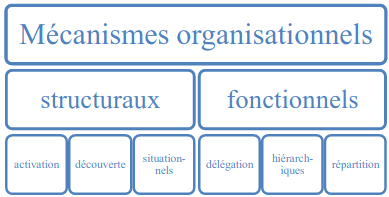
\includegraphics[width=8cm]{images/meca_orga.png}
            Peut être utile au moment de créer les jeux expérimentaux.
            \\
            \hline
            Une architecture d’agent BDI basée sur la théorie desfonctions de croyance : application à la simulation du comportement des agriculteurs
            &
            & Bon rappel avec exemple sur le fonctionnement des agents BDI, avec un exemple concret. \\
            \hline
        \end{tabular}
    \end{center}
    \end{table}


    \newpage
    \begin{table}[h]
        \begin{center}
        \begin{tabular}{|p{0.3\textwidth}|p{0.2\textwidth}|p{0.5\textwidth}|}
            \hline
            Intentional forgetting in distributed AI
            &
            & Dans les cas où il faut bcp (trop) d'infos pour traiter un pb, les SMA vont souvent distribuer le problème afin de réduire sa complexité. (à creuser : $https://www.researchgate.net/publication/326200455_Self-Organizing_Multiagent_Negotiations_Cooperation_and_Competition_of_Concurrently_Acting_Agents_with_Limited_Knowledge$). 
            Deux cas d'information overload (IO) : dimension qualitative, trop d'info car environnement trop riche -> agent spécialisés. Dimension quantitative, problème de la cpondance des informations, les agents peuvent s'échanger des infos fausses ou obsolètes -> bonne coordination.
            Compromis à trouver pour e savoir commun : en avoir permet une meilleure coordo et + de redondance, moins de risque de perte de savoir utile, mais trop entraine des IO. 
            Principe de "team cognition", quand le savoir est partagé entre agents spécialisés. Team coalition : agents avec des capacités hétérogènes. Team formation : capacités homogènes. Du coup leur Intentional Forgetting sert + à une réorganisation du savoir.
            Les agents utilisés sont des "discourse agents" (à creuser), une variante de BDI.
            Pour définir les agents, on a l'ensemble des actions, et pour chaque agent un sous ensemble représentant les actions qu'il est autorisé à utiliser en fonction de son rôle dans l'équipe. En plus de BDI, les agents ont aussi un ensemble de plans "capability", représentant l'ensemble des plans qu'ils sont capables de réaliser.
            Une "transactive memory" permet de savoir qui est capable de quoi. Elle est individuelle, mais dans un monde idéal, tout le monde a une vision exacte des capacités de chacun, c'est donc un savoir partagé. Un modèle mental individuel également permet de savoir qui a quelles intentions. De la même manière, dans un monde parfait, il y a consensus là-dessus, et donc ce savoir individuel devient un savoir partagé.
            Quand un agent apprend ou oublie qqc, il suffit de le faire savoir à tlm pour qu'ils mettent leur TM à jour.
            \\
            \hline
            Description logics, Franz Baader, Ian Horrocks and Ulrike Sattler (2008)
            &
            & Analogie (personnelle, pas dans le papier), Tbox = classe, Abox = objet, instance. Dans le papier, Tbox = schema, Abox = data.
            Tbox est appelée "definitorial" ssi elle ne contient que des définitions, et qu'il n'y a pas de cycle.
            ALC une DL très utilisée, qui donne les bases, et a connu des extensions (par exemple "number restriction" pour ajouter des nombres à des définitions). Fait une comparaison entre DL, logique de 1er ordre et logique modale. A continuer.
            \\
            \hline
            Towards Simulation-Based Role Optimization in Organizations
            &
            & Tente de résoudre le problème Job-Shop-Scheduling avec une approche multi-agent. Cherche avant tout à maximiser la répartition initiale des rôles, donc pas forcément utile pr moi.\\
            \hline
            PR-OWL: A Bayesian Ontology Language for the Semantic Web
            &
            & Présente différentes alternatives bayésiennes. Les réseaux bayésiens classiques ne sont pas assez expressifs. L'approche proposée se base sur la logique MEBN (Multi Entity Bayesian Network), qui combine probas et logique de premier ordre. Certaines requêtes peuvent toutefois s'avérer indécidables. A continuer après + de recherches sur réseaux bayésiens\\
            \hline
            Bayesian Network (Pearl et Russell, 2000)
            &
            & Apprendre dans un tel réseau est un peu comme entrainer un NN : c'est faire varier les probas entre les entités (les poids des liens entre les noeuds). Un réseau causal est un réseau où les parents d'un noeud sont sa cause directe. Si on fixe la valeur d'un noeud, on retire alors le lien avec ses parents. Vieux, donc probablement plus à jour, mais explique bien la base des réseaux bayésiens.
            \\
            \hline
            Advances in Bayesian network modelling: Integration of modelling technologies
            &
            & Présente de nombreux champs d'applications où des BN ont été utilisés. Peut être intéressant : agent based modeling. IBN, des BN intégrés à d'autres modèles. Ajd, ils sont surtout statiques (réalisés par des experts).
            \\
            \hline


        \end{tabular}
    \end{center}
    \end{table}


    \newpage
    \begin{table}[h]
        \begin{center}
        \begin{tabular}{|p{0.3\textwidth}|p{0.2\textwidth}|p{0.5\textwidth}|}
            \hline
            Bayesian or biased? Analytic thinking and political belief updating
            & 
            & Etude de psycho cognitive. On pose des questions orientées politiquement à des personnes. Après chaque réponse, un signal indique vrai/faux. Ils ont été informés que ce signal donnait la bonne réponse 2 fois sur 3. On s'intéresse alors à comment les gens ont update leurs croyances, en leur posant les mêmes questions une seconde fois. Intéressant, mais se focalise surtout sur des idées polémiques, et donc des raisonnements motivés, pas des cas plus basiques. Etablit une corrélation (faible, mais significative statistiquement) entre score au RCT et capacité à update ses croyances en restant proche d'un modèle bayésien.
            \\
            \hline
            Bayesian models of cognition (2008)
            &
            & Cite au début bcp de modèles bayésiens utilisés en science cognitive, peut être utile. Un peu technique, mais présente différentes approches bayésiennes, dont les BNs, et leurs fondements mathématiques.
            \\
            \hline
            Bayesian theories of conditioning in a changing world
            &
            & Papier qui cite des études montrant que chez les animaux, la surprise (par exemple, conditionner l'animal à lui donner de la bouffe après une sonnerie, mais au bout d'un moment lui envoyer un choc électrique), et donne une interprétation bayésienne à ce fait (en gros, surprise -> grosse incertitude sur leurs croyances actuelles -> plus gros updates dans les probas de leurs croyances).
            \\
            \hline

            The case for Motivated Reasonning
            &
            & Présente le phénomène de "raisonnement motivé". Historiquement, une thèse concurrente était de dire que simplement, pour certains individus, certaines croyances étaient + plus plausibles au vu de leurs croyances initiales (prior believes).
            \\
            \hline


            MEBN: A language for first-order Bayesian knowledge bases
            &
            & (à lire)
            \\ 
            \hline
            The Bayesian Ontology Language
            &
            & (à lire)
            \\
            \hline
        \end{tabular}
    \end{center}
    \end{table}

    Regarder les recherches du laboratoire de psychologie et neurocognition

    \nocite{*}
    \bibliographystyle{plain}
    \bibliography{bibli}
\end{document}